\documentclass{beamer}

\usetheme[secheader]{Boadilla}
\usecolortheme{seahorse}
\usepackage[spanish]{babel} 		% {Con estos dos anda
\usepackage[utf8]{inputenc} 		% todo lo que es tildes y ñ}
\usepackage{graphicx}

\title{Pedí un taxi ahora con: TAXINOW}
\author{Martín Carreiro - Pablo Rago - Juan Manuel Tastzian}
\date{2 de Julio de 2014}
\institute[2014]{Facultad de Ciencias Exactas y Naturales}

\begin{document}

\frame{\titlepage}

\section{Sobre TaxiNow}

\frame {
	\frametitle{¿Qué es TaxiNow?}
	TaxiNow es una aplicación con dos enfoques principales
	\begin{itemize}
		\item<2-> Enfoque de taxista.
		\item<3-> Enfoque de pasajero de un taxi.
	\end{itemize}
}

\frame {
	\frametitle{¿Qué es TaxiNow?}
	Elección de enfoque:
	\begin{center}
		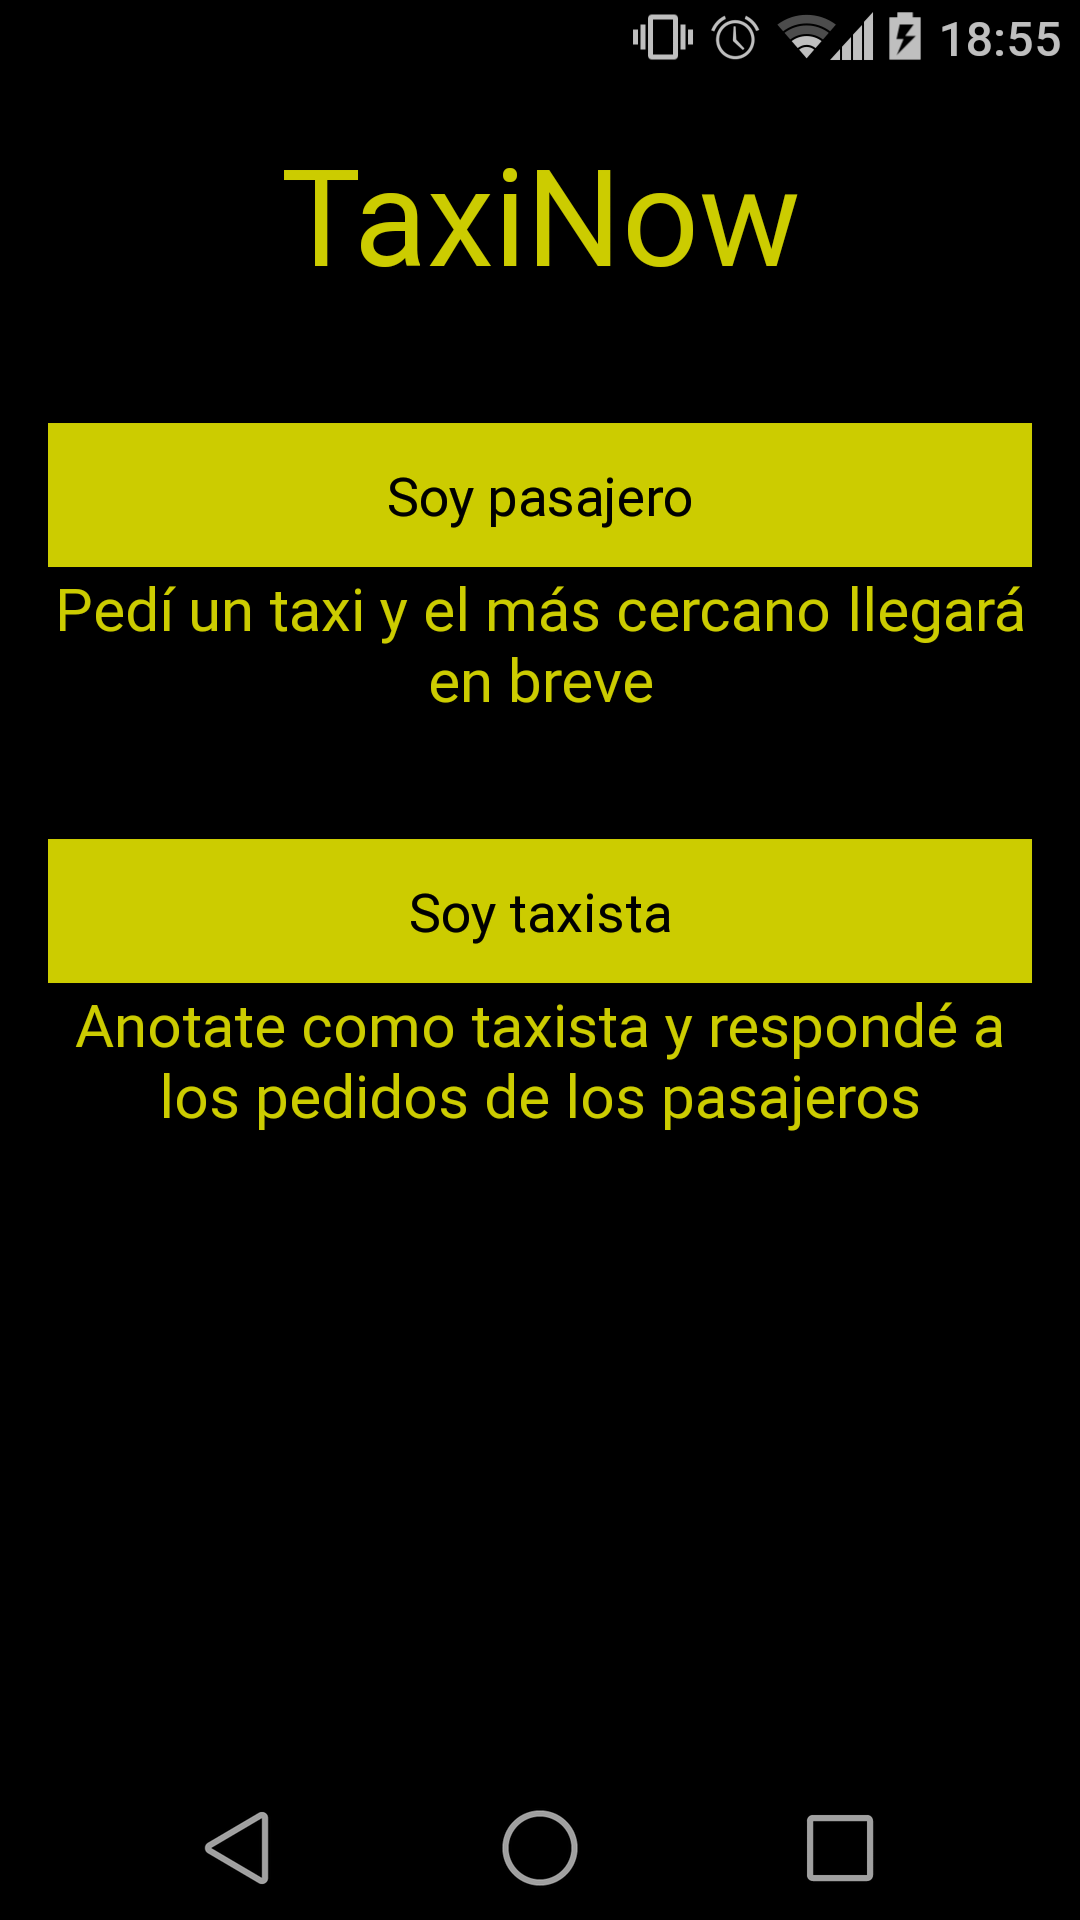
\includegraphics[scale=0.1]{./screenshots/01_UserTypeChoosing.png}	
	\end{center}
}

\frame {
	\frametitle{Enfoque de taxista}
	Un taxista puede:
	\begin{itemize}
		\item <2-> Registrarse en la aplicación.
		\item <3-> Completar su perfil.
			\begin{itemize}
				\item <4-> Publicar una foto de su vehículo.
				\item <5-> Registrar su marca, modelo y patente del taxi.
			\end{itemize}
		\item <6-> Esperar que lleguen viajes.
		\item <7-> Aceptar o ignorar viajes.
	\end{itemize}
}

\frame {
	\frametitle{Enfoque de taxista}
	\begin{center}
		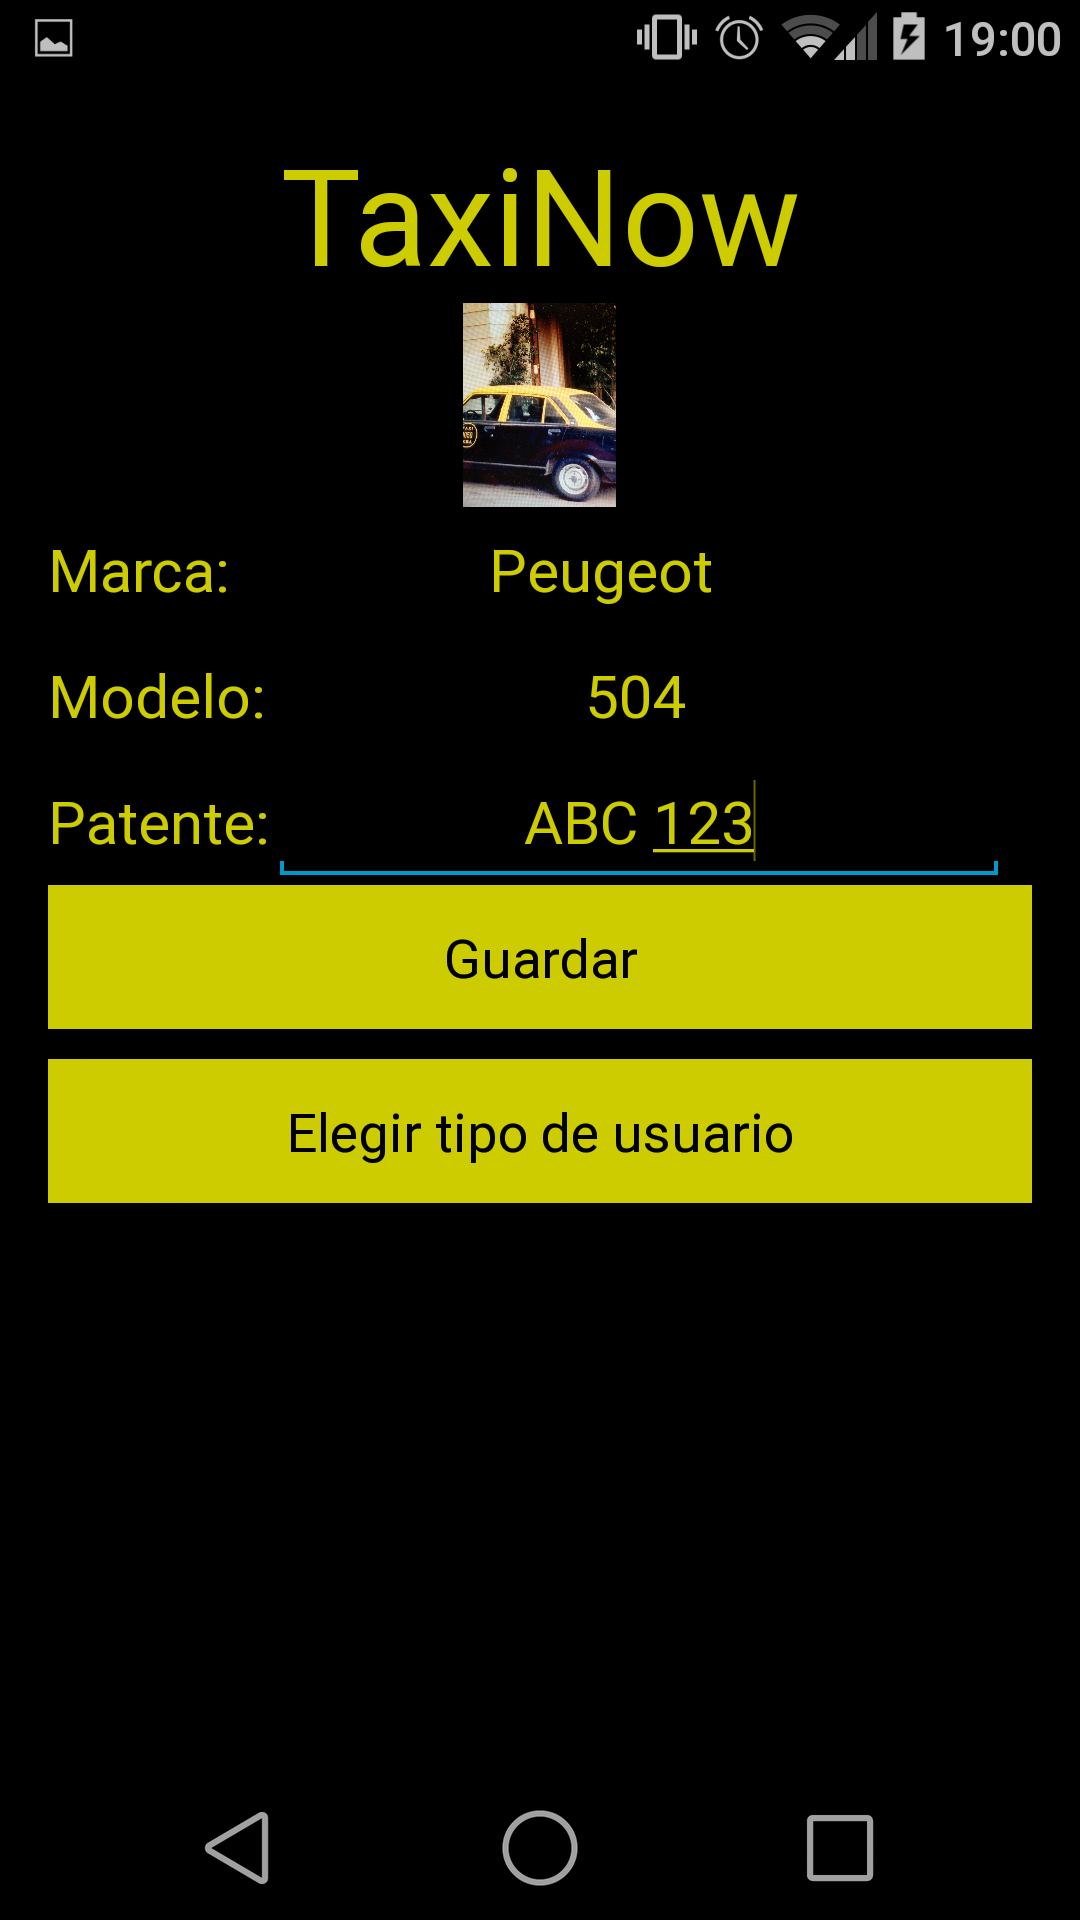
\includegraphics[scale=0.1]{./screenshots/02_TaxiConfig.png}	
	\end{center}
}

\frame {
	\frametitle{Enfoque de pasajero}
	Un pasajero puede:
	\begin{itemize}
		\item <2-> Registrarse en la aplicación.
		\item <3-> Decir a donde quiere ir y pedir un taxi.
	\end{itemize}
}

\frame {
	\frametitle{Enfoque de pasajero}
	\begin{center}
		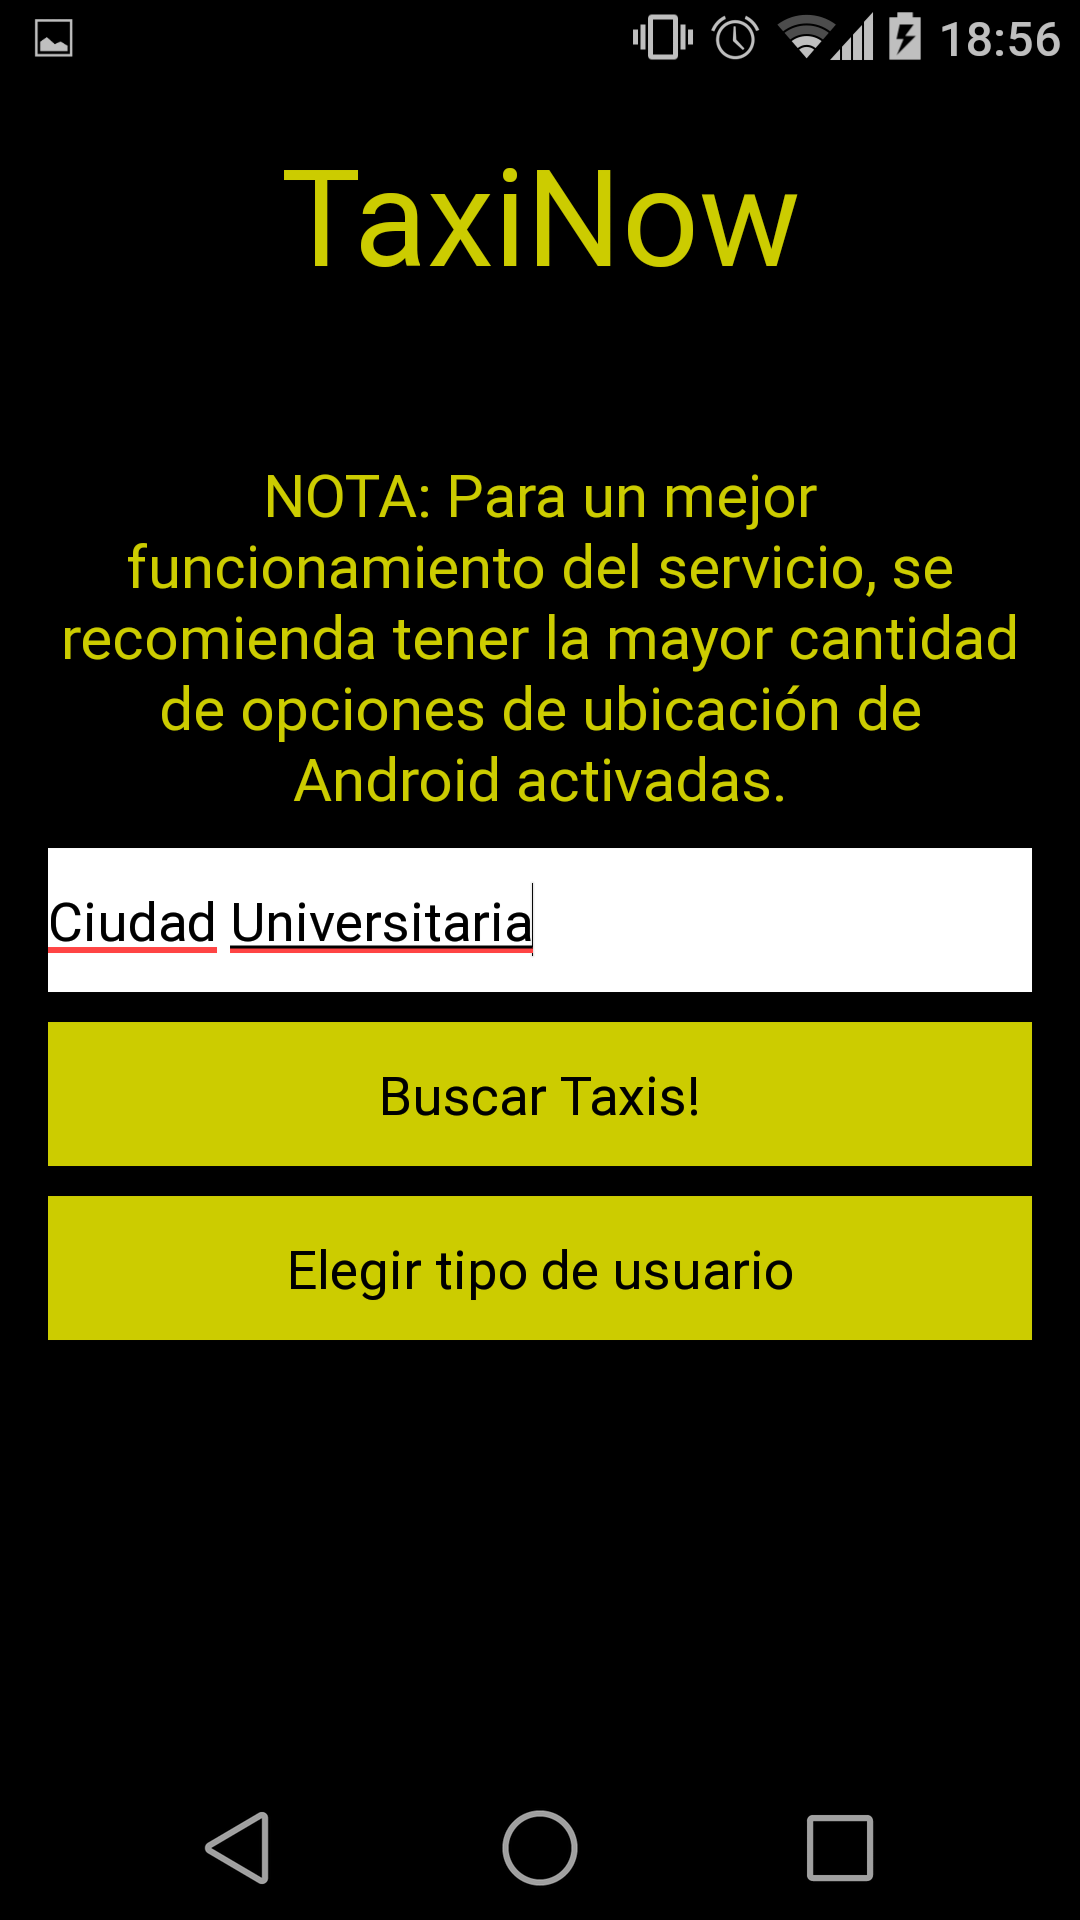
\includegraphics[scale=0.1]{./screenshots/05_PassengerCompleta.png}	
	\end{center}
}

\section{Flujo de la aplicación}

\frame {
	\frametitle{Ejemplo de taxista}
	\begin{itemize}
		\item <1-> Primero el taxista se registra.
		\item <2-> Completa la marca, modelo y patente del auto (que luego se enviará como información de reconocimiento al pasajero).
		\item <3-> Finalmente, como detalle opcional, se permite acceder a la cámara y sacar una foto del taxi para agregar a su perfil de taxista (se guarda en la memoria del teléfono).
		\item <4-> Esto fue mostrado antes.
	\end{itemize}
}

\frame {
	\frametitle{Ejemplo de taxista}
	\begin{itemize}
		\item <1-> Una vez registrado, el taxista, entra en modo de espera.
		\item <2-> En el mismo le empiezan a llegar los viajes de los pasajeros que hagan los pedidos.
		\item <3-> El taxista puede aceptar o rechazar el viaje.
		\item <4-> A continuación, un ejemplo de esto.
	\end{itemize}
}

\frame {
	\frametitle{Esperando viajes (Taxista)}
	\begin{center}
		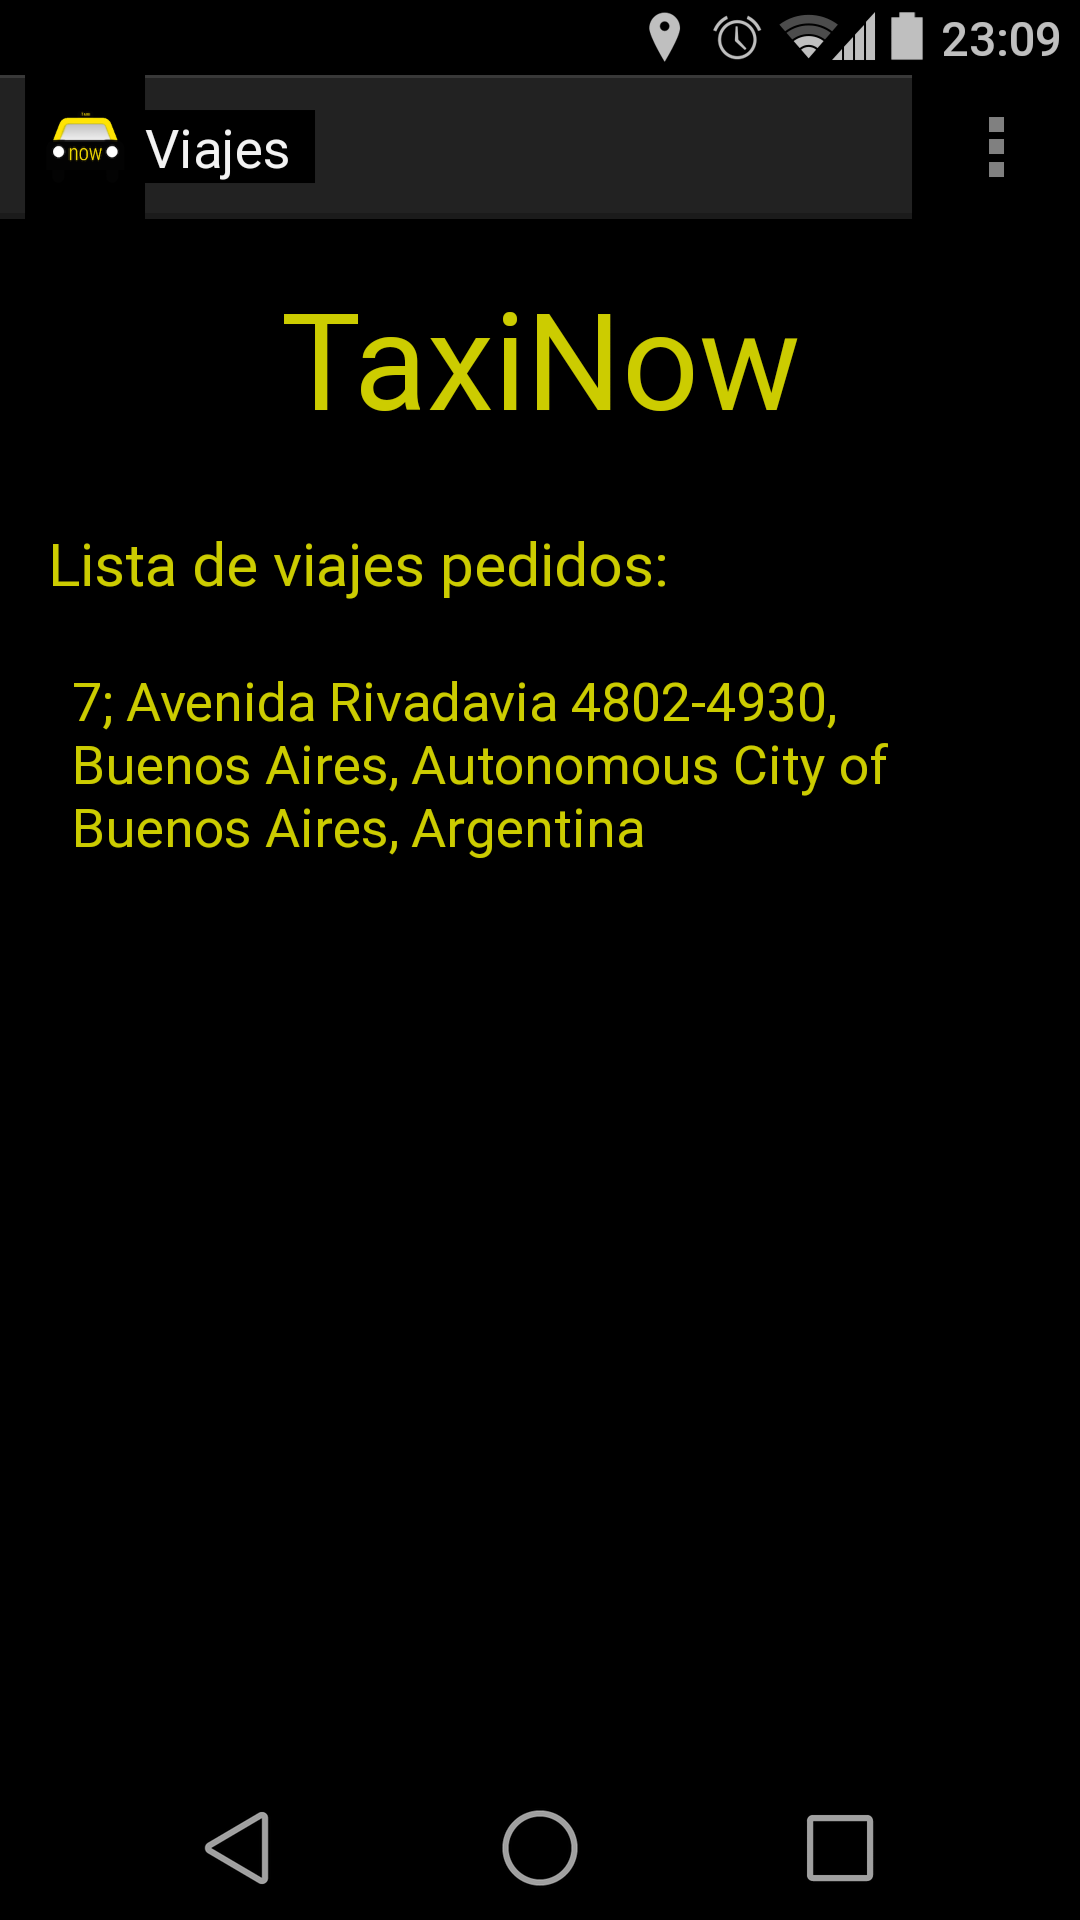
\includegraphics[scale=0.1]{./screenshots/03_TaxiAvailable.png}	
	\end{center}
}

\frame {
	\frametitle{Ejemplo de taxista}
	En este momento se puede minimizar la aplicación y seguir utilizando el teléfono normalmente, que si llega un viaje, aparecerá la notificación pertinente.
}

\frame {
	\frametitle{Notificaciones (Taxista)}
	\begin{center}
		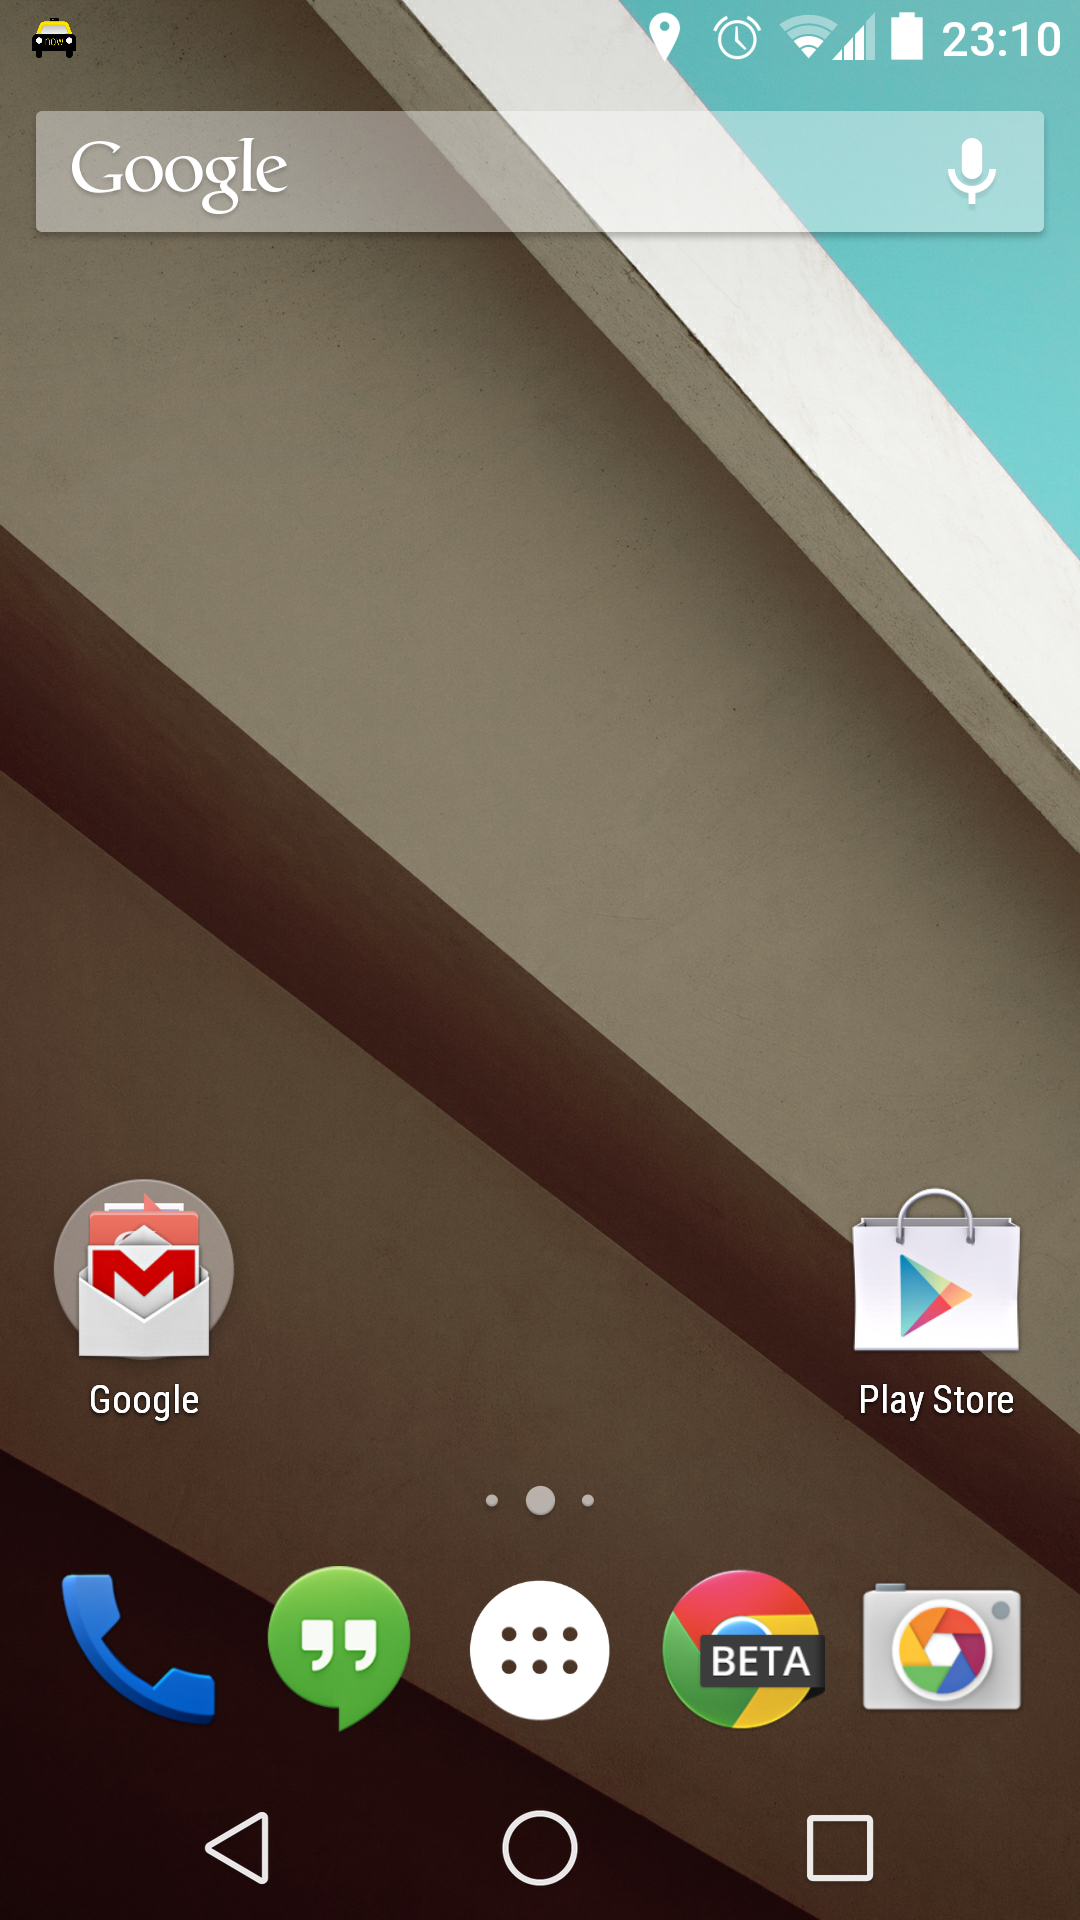
\includegraphics[scale=0.1]{./screenshots/NotificationCollapsed.png}
		\hspace{1cm}
		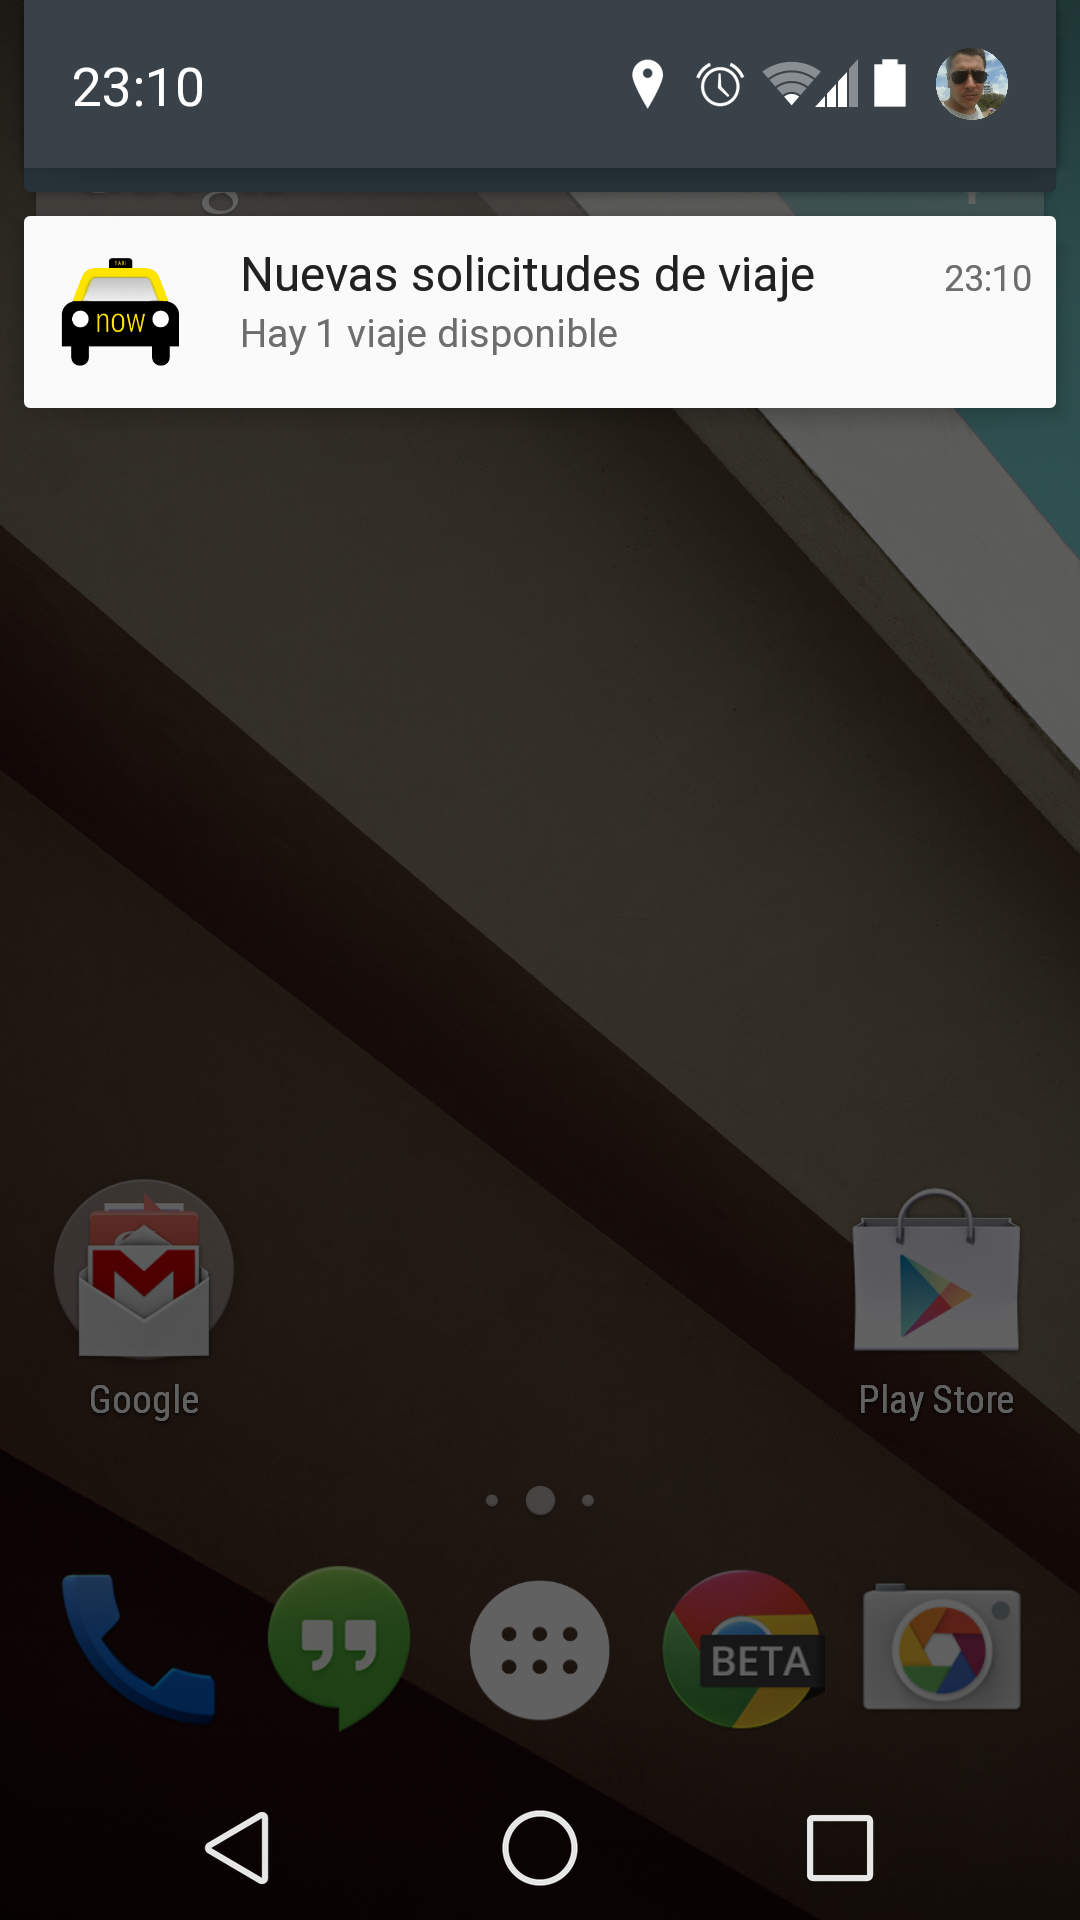
\includegraphics[scale=0.1]{./screenshots/NotificationExpanded.png}
	\end{center}
}

\frame {
	\frametitle{Y cada tanto, se filtra alguna alegría}
	\begin{center}
		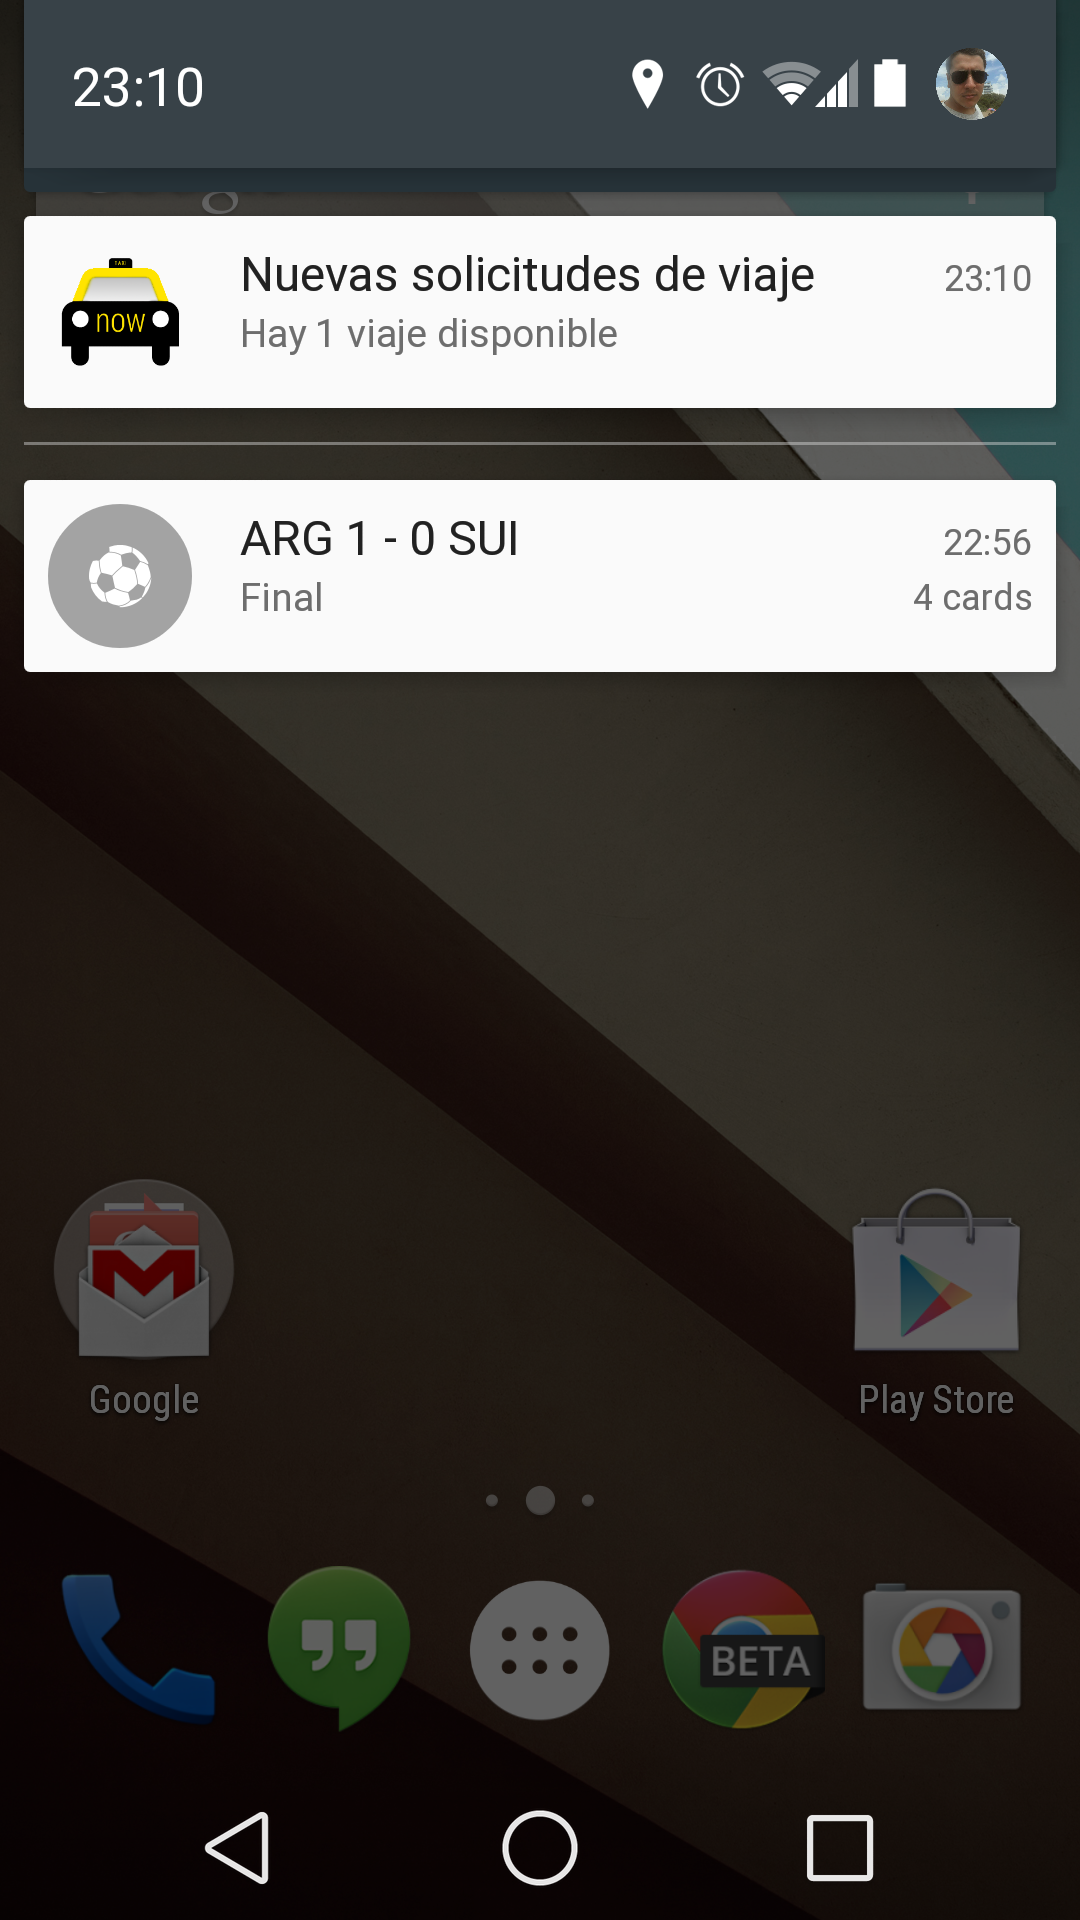
\includegraphics[scale=0.1]{./screenshots/NotificationExpandedMatch.png}
	\end{center}
}

\frame {
	\frametitle{Ejemplo de taxista}
	\begin{itemize}
		\item <1-> Finalmente, presionando en un viaje, el taxista acepta el mismo.
		\item <2-> En este momento, el taxista pasa a estar ``no disponible'' para el resto de los pasajeros.
		\item <3-> Para no recibir notificaciones inútiles/distractoras mientras está ocupado con otro viaje.
		\item <4-> Existe un botón para finalizar el viaje y volver a estado ``disponible'' para recibir nuevos viajes.
	\end{itemize}
}

\frame {
	\frametitle{Viaje confirmado (Taxista)}
	\begin{center}
		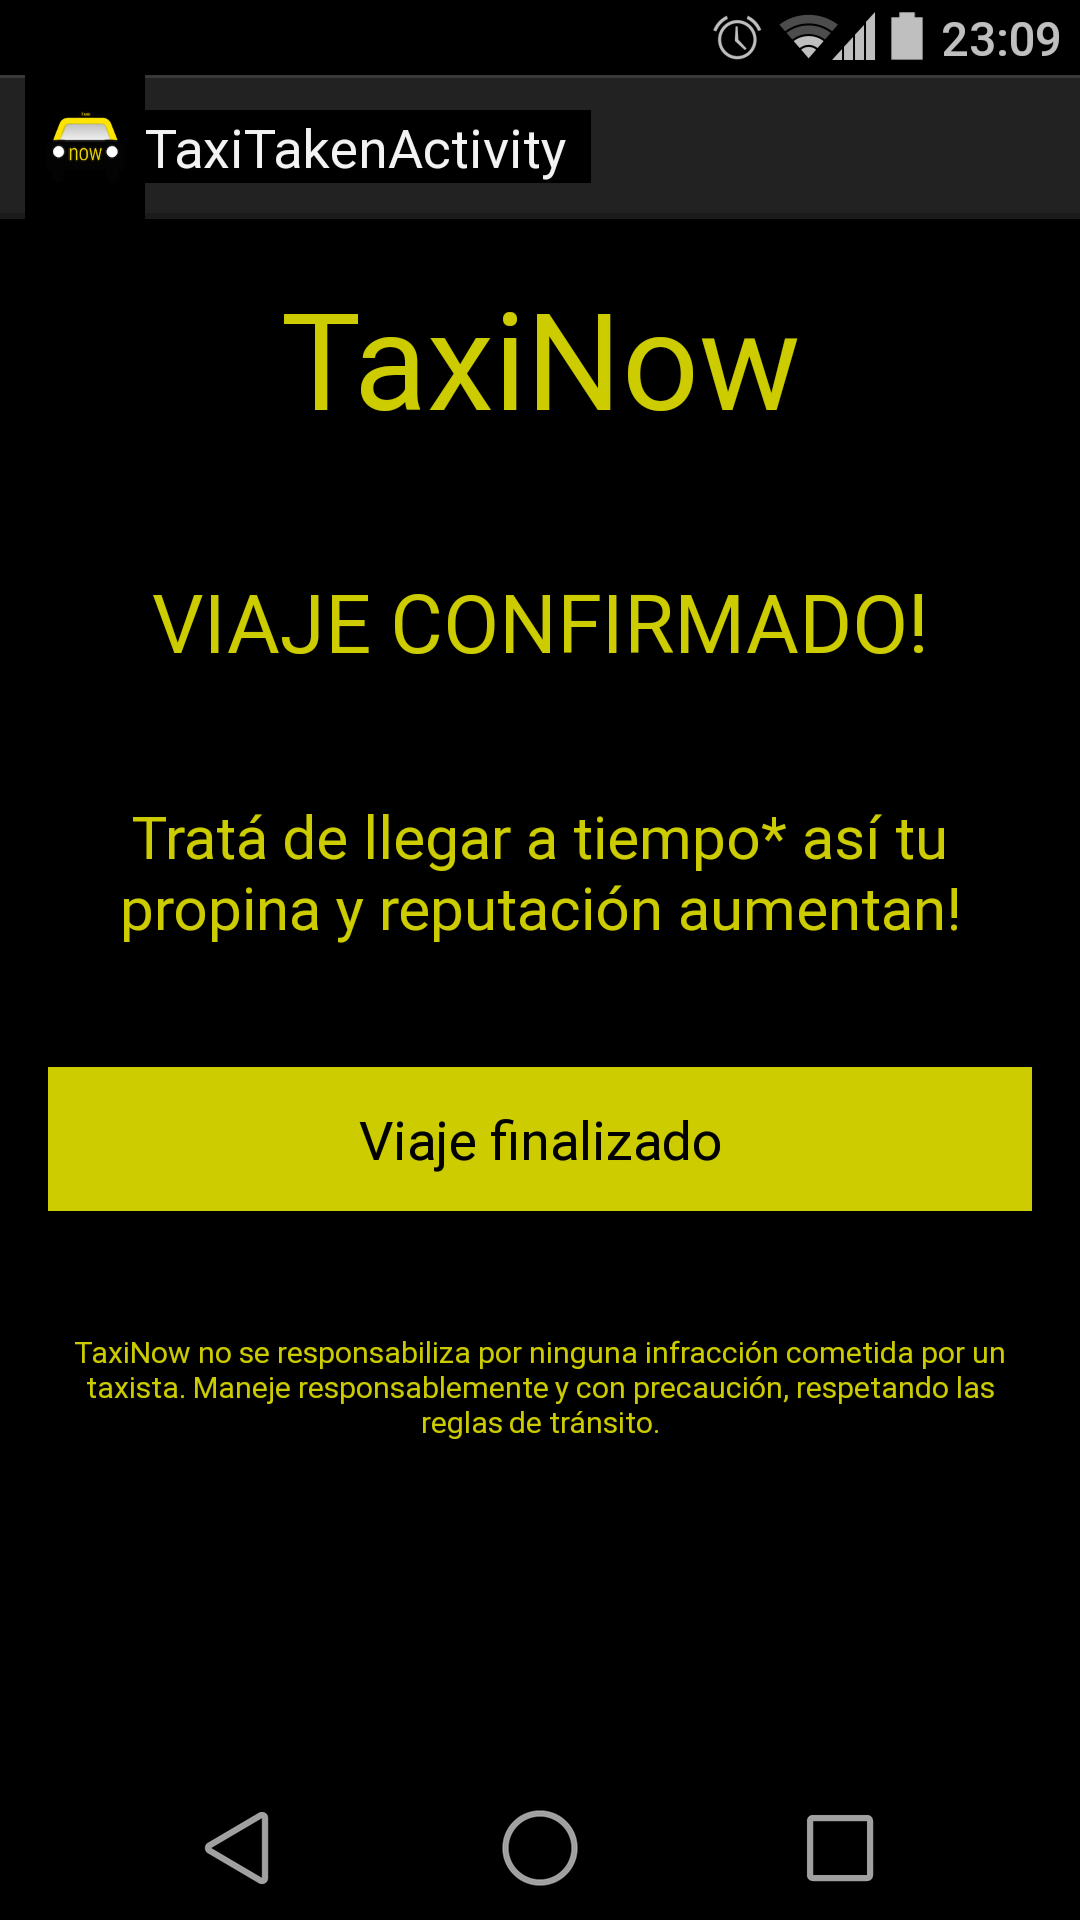
\includegraphics[scale=0.1]{./screenshots/04_TripConfirmed.png}
	\end{center}
}

\frame {
	\frametitle{¿Y que pasa del otro lado?}
	\begin{itemize}
		\item <1-> Esto termina el flujo del lado del taxista, pero...
		\item <2-> ...¿que pasa con el pasajero, mientras?
	\end{itemize}
}

\frame {
	\frametitle{Ejemplo de pasajero}
	El pasajero elige hacia donde ir y presiona el botón para comenzar la búsqueda de taxis.
}

\frame {
	\frametitle{Eligiendo destino (pasajero)}
	\begin{center}
		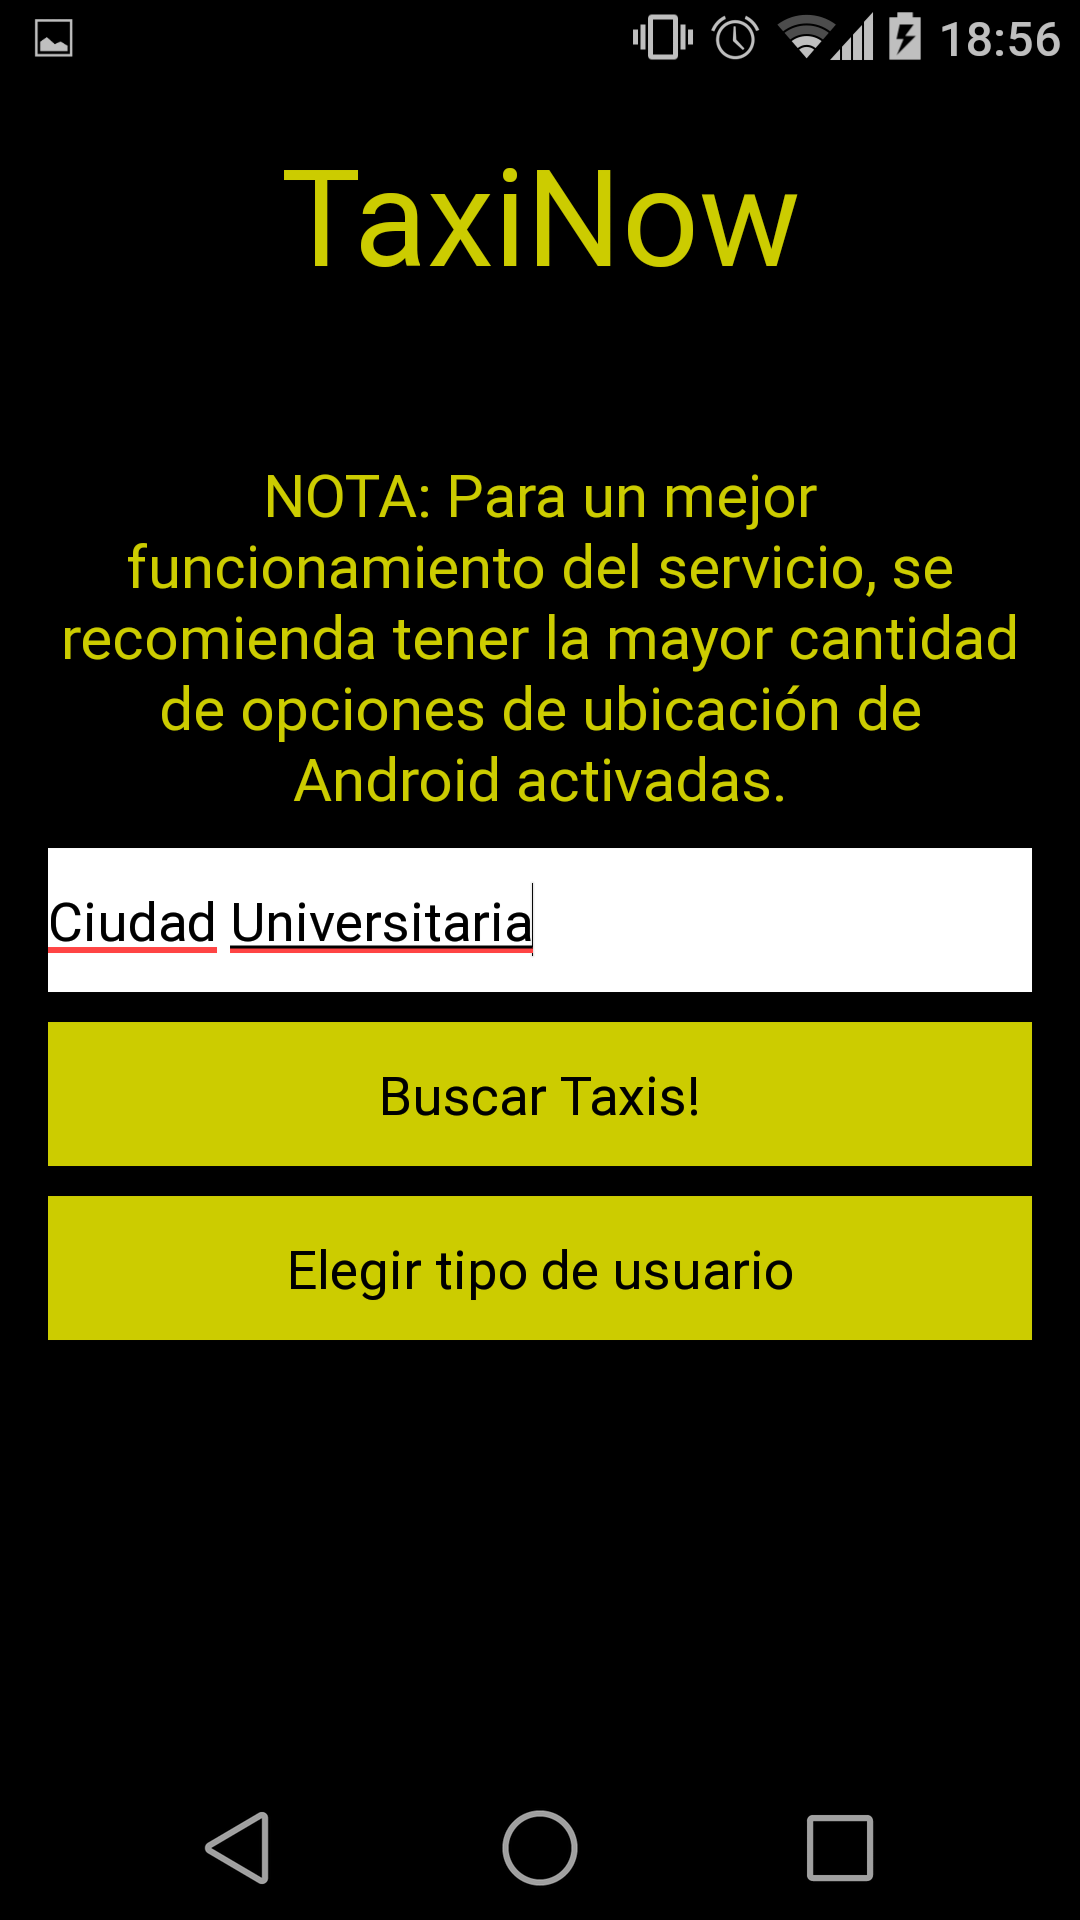
\includegraphics[scale=0.1]{./screenshots/05_PassengerCompleta.png}	
	\end{center}
}

\frame {
	\frametitle{Ejemplo de pasajero}
	\begin{itemize}
		\item <1-> Luego de esto, el pasajero espera unos segundos mientras se realiza la búsqueda de taxistas.
		\item <2-> Si no se encuentra un taxista disponible en 60 segundos, la búsqueda termina y se puede reiniciar.
		\item <3-> Si se encuentra un taxista disponible, el pasajero recibe la confirmación y los datos del taxi, para poder reconocerlo cuando éste llega (son los datos ingresados por el taxista en su registración).
	\end{itemize}
}

\frame {
	\frametitle{Esperando confirmación de algún taxista}
	\begin{center}
		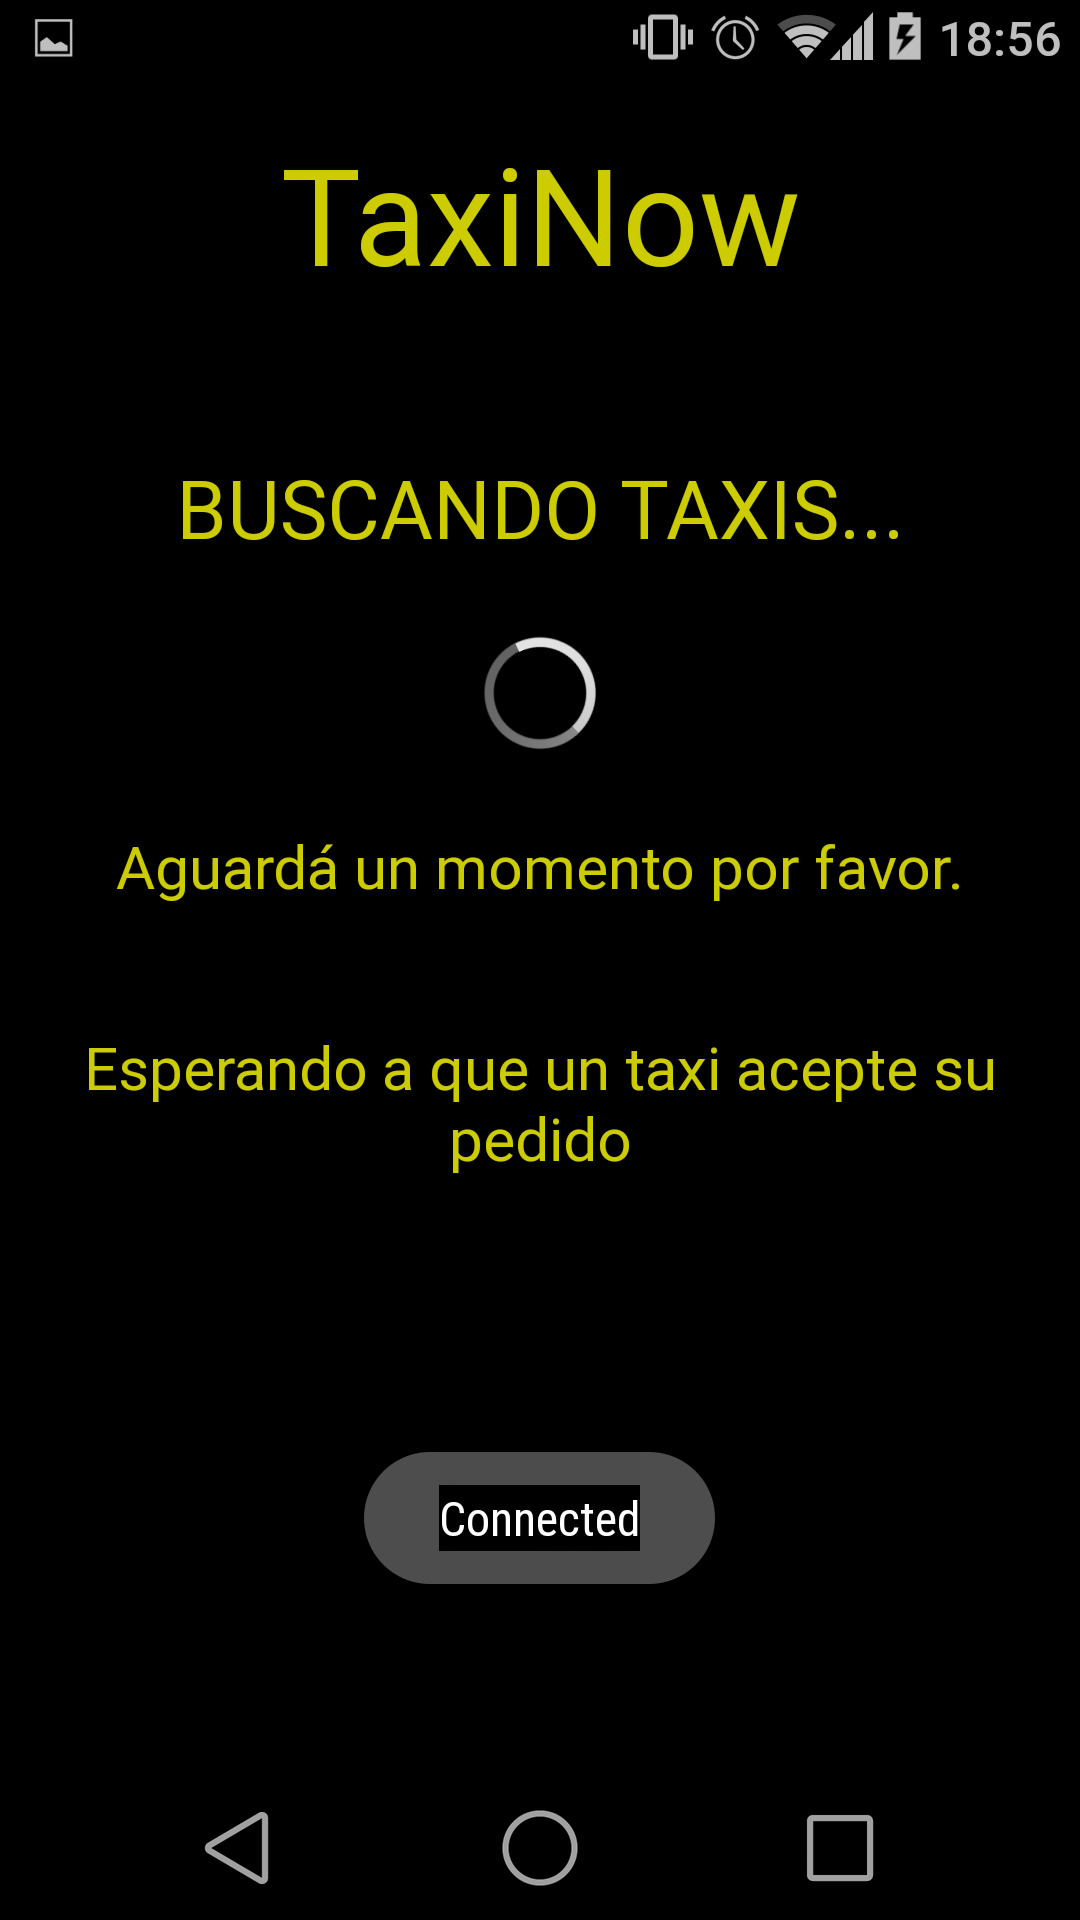
\includegraphics[scale=0.1]{./screenshots/06_SearchingTaxis.png}	
	\end{center}
}

\frame {
	\frametitle{Viaje confirmado (pasajero)}
	\begin{center}
		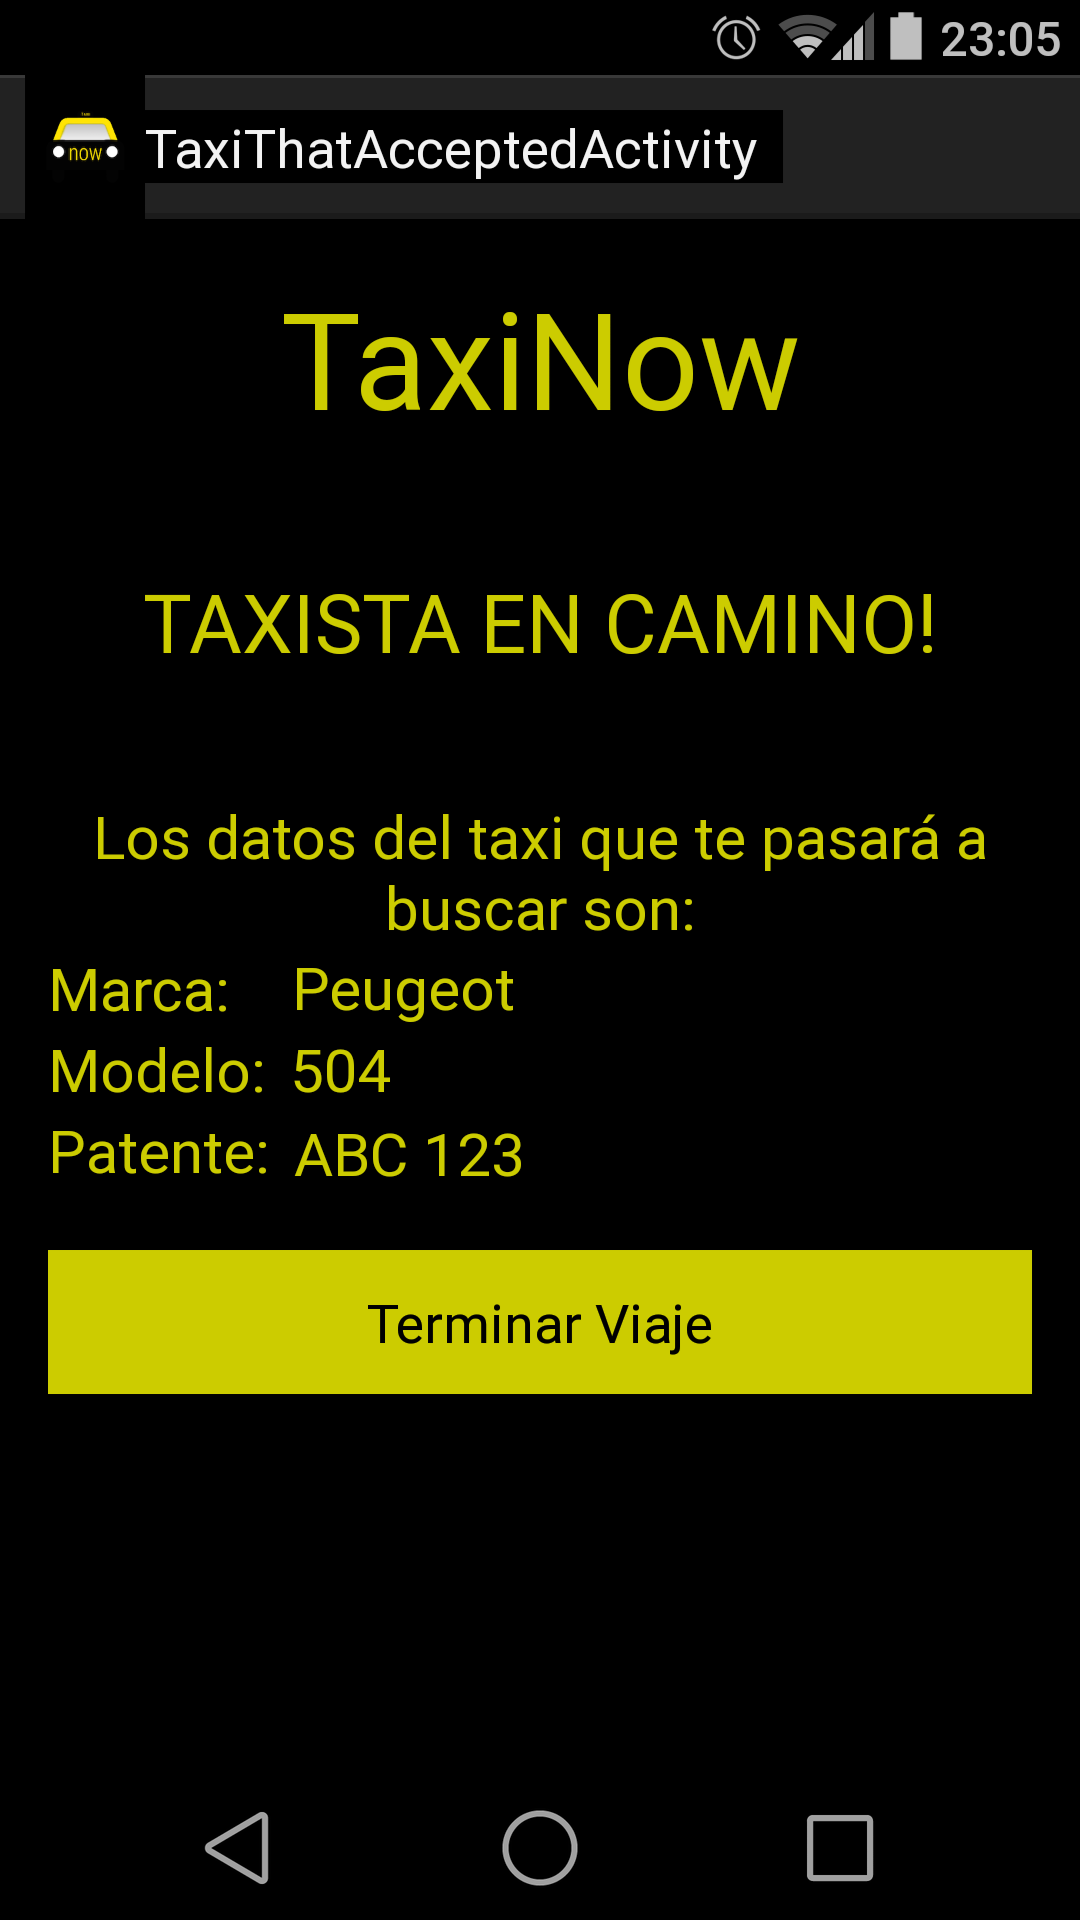
\includegraphics[scale=0.1]{./screenshots/07_TaxiTaken.png}	
	\end{center}
}

\frame {
	\frametitle{Posibles mejoras}
	Esto termina la demostración del flujo actual de la aplicación. Nos hubiese gustado poder implementar las siguientes mejoras o características:
	\begin{itemize}
		\item <2-> Si varios taxistas aceptan el viaje, que el pasajero pueda elegir uno, ya sea por ubicación, preferencia de auto que tiene o rating.
		\item <3-> Hablando de rating: sistema de rating colectivo de taxistas. Poder puntuar el taxista (ya sea por eficiencia, velocidad, comodidad, habilidades, etc.) luego de terminar el viaje.
		\item <4-> Que el pasajero pueda elegir hasta que distancia acepta que un taxi se postule para el viaje (si estás en Belgrano y te acepta un taxi de Liniers, no nos parece que ganes mucho en comodidad/tiempo...)
		\item <5-> Integrar la API de Google Maps, para que tanto al taxista como al pasajero, le muestre visualmente donde se ubica el otro, para una comprensión más directa de las distancias y la ubicación.
		\item <6-> Mejorar la estética y usabilidad general de la aplicación.
	\end{itemize}
}

\end{document}